\cleardoublepage

\section{Allgemeine Mobilgeräte-Analyse}
\label{analyse}
Bevor in der Bachelorarbeit damit begonnen werden konnte, Auswertungen über 
Mobilgeräte vorzunehmen, musste die allgemeine Verteilung von Smartphones
auf dem Schweizer Mark analysiert werden. 
Dafür wurden Zahlen vom Bundesamt für Statistik aus dem Jahr 2019 ausgewertet
und ergänzend Verkaufszahlen und Nutzerstatistiken bekannter Hersteller gesucht.

\subsection{Smartphones}
In der Schweiz gibt es im Jahr $2020$ ungefähr $6.8$ Millionen Personen,
die ein Smartphone besitzen.
Prognosen sagen aus, dass bis im Jahr $2025$ über $7$ Millionen Personen
ein Mobilgerät besitzen werden. 
In der Abbildung~\ref{figure:AnzSmartphoneUser} sind die statistischen
Zahlen und Prognosen bis zum Jahr $2022$ ersichtlich.    

\begin{figure}[h!]
    \centering
    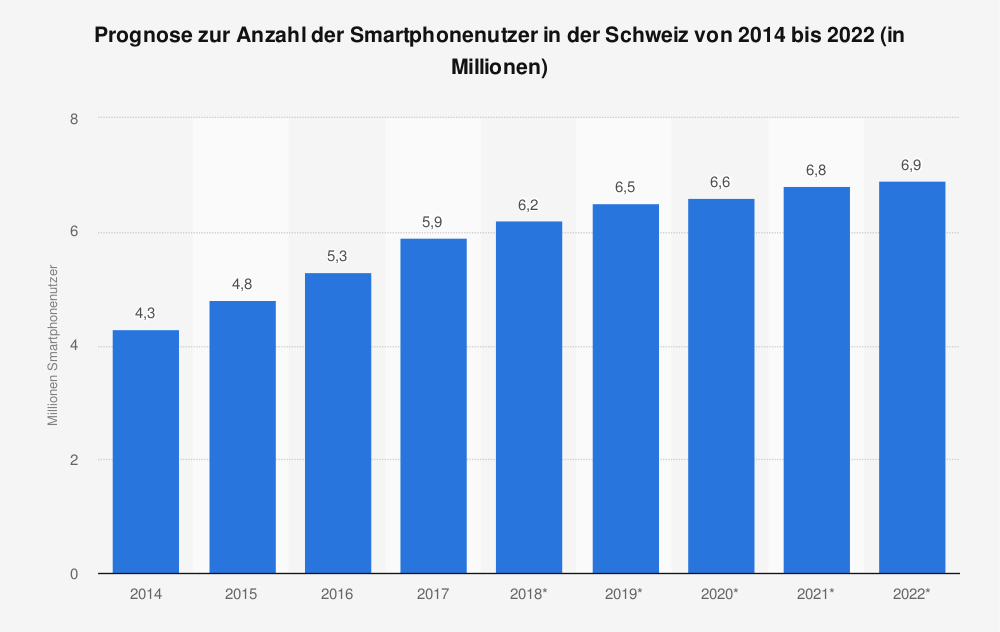
\includegraphics[width=1\linewidth]{Analyse/anz_smartphone_nutzer_prognose.png}
    \caption{Anzahl Smartphone User in der Schweiz}
    \label{figure:AnzSmartphoneUser}
\end{figure}

\clearpage
    
Um die Nutzung der Mobilgeräte noch weiter zu unterteilen, wurde eine 
Aufteilung nach Betriebssystem der Smartphones durchgeführt.
Die Ergebnisse sind in der Abbildung~\ref{figure:SmartphoneBsys} aufgezeigt.

\begin{figure}[h!]
    \centering
    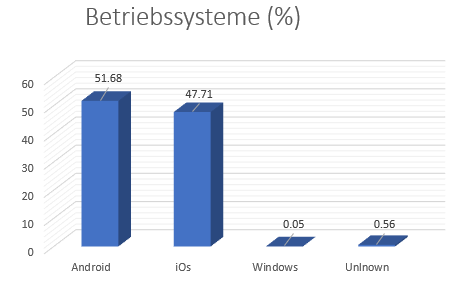
\includegraphics[width=1\linewidth]{Analyse/smartphone_bsys.PNG}
    \caption{Verteilung der Betriebssysteme}
    \label{figure:SmartphoneBsys}
\end{figure}

Hauptsächlich sind die beiden Betriebssysteme Android und IOS mit zusammen
über $99$ Prozent Marktanteil im Jahr $2019$ vertreten.

\clearpage

IOS wird nur von IPhones verwendet, aber Android-Geräte lassen sich noch weiter
nach Hersteller unterteilen. 

In der Abbildung~\ref{figure:SmartphoneHersteller} ist die Verteilung
nach Hersteller im Jahr $2019$ aufgelistet.

\begin{figure}[h!]
    \centering
    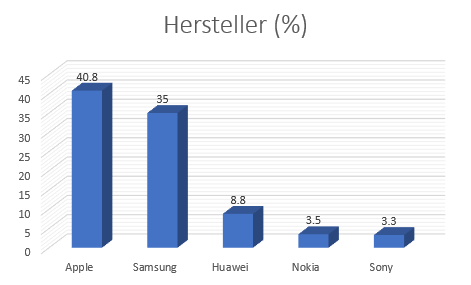
\includegraphics[width=1\linewidth]{Analyse/smartphone_hersteller.PNG}
    \caption{Verteilung der Hersteller}
    \label{figure:SmartphoneHersteller}
\end{figure}

Die meistverwendeten Smartphones sind entweder IPhones oder Samsung-Geräte.
Huawei hat mit $8.8$ Prozent einen eher kleinen Marktanteil und wird in naher Zukunft
ein eigenes Betriebssystem für seine Geräte anbieten, da der Hersteller 
aufgrund diverser Privatsphäreanschuldigungen in der USA auf schwarzen Liste 
steht. 

\clearpage

\subsection{Auswahl der Mobilgeräte}
Basierend auf den gewonnenen Erkenntnissen konnten die für die Versuche
benötigten Mobilgeräte ausgewählt werden.

In der Analyse der beiden Betriebssysteme IOS 
(Siehe Abschnitt~\ref{section:iosanalysis}) und Android
(Siehe Abschnitt~\ref{section:androidanalysis}) hat sich gezeigt, dass
IOS-Geräte ab IPhone 8 und Android-Geräte mit der Android-Version 9 oder neuer
für die Versuche in Betracht gezogen werden. 
Nachfolgend sind die Geräte aufgelistet.

\paragraph{IOS-Geräte}
\begin{itemize}
    \item IPhone 8
    \item IPhone X
    \item IPhone XR
    \item IPhone XS
    \item IPhone 11
    \item IPhone 11 Pro
    \item IPhone SE
\end{itemize}

\paragraph{Samsung-Geräte}
\begin{itemize}
    \item Samsung Galaxy S8
    \item Samsung Galaxy S9
    \item Samsung Galaxy S9+
    \item Samsung Galaxy S10
    \item Samsung Galaxy S10 light
    \item Samsung Galaxy S20
    \item Samsung Galaxy S20+
    \item Samsung Galaxy S20 ultra
\end{itemize}

\paragraph{Google-Geräte}
\begin{itemize}
    \item Pixel 3
    \item Pixel 3 XL
    \item Pixel 3a
    \item Pixel 3a XL
    \item Pixel 4
    \item Pixel 4 XL
\end{itemize}

\paragraph{Weitere Hersteller}
\begin{itemize}
    \item OnePlus 7T 
    \item Oneplus 7T Pro 
    \item Oneplus 8
    \item Oneplus 8 Pro
    \item Huawei P20
    \item Huawei P30
    \item Fairphone 3
    \item Fairphone 3+
    \item Weitere, falls Android-Version 9 oder neuer
\end{itemize}

Die Auflistung zeigt nur die Geräte, welche für die Versuche in 
Betracht gezogen werden. Die tatsächlich verwendeten Geräte 
werden im Kapitel~\ref{chapter:experiments}: Versuche aufgelistet.

\clearpage